\documentclass[12pt, oneside, a4paper]{report}
\usepackage{hyperref,graphicx}
\usepackage[top=3cm, bottom=3cm, left=3cm, right=3cm]{geometry}
\usepackage{setspace}
\usepackage{fontspec}
\usepackage{float}
\usepackage{color}
\usepackage[usenames,dvipsnames,svgnames,table]{xcolor}
\usepackage{xunicode}
\usepackage{array}
\usepackage{booktabs,bookmark}
\usepackage{longtable}
\usepackage{ragged2e}
\usepackage[font={footnotesize,it}]{caption}
\usepackage{parskip}
\usepackage{amsmath}
\usepackage{amssymb}
\usepackage{bm}
\usepackage{textcomp}
%\usepackage[customcolors]{hf-tikz}
\usepackage{xspace}
\usepackage[Greek,Latin]{ucharclasses}
\usepackage{xltxtra}
\usepackage{xgreek} 
\usepackage[sort&compress,numbers]{natbib}
\usepackage{float}
\usepackage{mathtools}

% \usepackage[utf8]{inputenc}

%\usepackage{minted}

\renewcommand{\labelenumii}{\theenumii}
\renewcommand{\theenumii}{\theenumi.\arabic{enumii}.}

%\floatname{algorithm}{Αλγόριθμος}
\renewcommand\figurename{Εικόνα}
%\renewcommand\tablename{Πίνακας}

\setTransitionsForGreek{\setlanguage{greek}}{\setlanguage{american}} % Instead of american, any other language can be used

\renewcommand\thesection{\arabic{section}}

\hypersetup{
 %bookmarks=true, % show bookmarks bar?
unicode=true, % non-Latin characters in Acrobat’s bookmarks
pdftoolbar=true, % show Acrobat’s toolbar?
pdfmenubar=true, % show Acrobat’s menu?
pdffitwindow=false, % window fit to page when opened
pdfstartview={FitH}, % fits the width of the page to the window
pdftitle={Stakeholder's Requirements Specification}, % title
pdfauthor={Daphne Tsolissou}, % author
pdfsubject={}, % subject of the document
pdfcreator={LaTeX}, % creator of the document
% pdfproducer={LateX}, % producer of the document
%pdfkeywords= % list of keywords
pdfnewwindow=true, % links in new window
colorlinks=false, % false: boxed links; true: colored links
linkbordercolor={1 1 1}, % color of internal links (change box color with linkbordercolor)
%citecolor=white, % color of links to bibliography
citebordercolor={1 1 1},
filecolor=magenta, % color of file links
urlcolor=cyan % color of external links
}

\setmainfont{Times New Roman}
\singlespacing
\frenchspacing
\setlength{\parindent}{0.6cm}
\setlength{\parskip}{0.5pt}

\begin{document}
%      \parbox[l]{\textwidth}{
\flushleft{\Huge{\textbf{Έγγραφο απαιτήσεων εμπλεκομένων μερών (StRS)}}}\\
\flushleft{\Huge{\textbf{Stakeholders Requirements Specification}}}\\
\flushleft{\footnotesize{ΠΡΟΣΑΡΜΟΓΗ ΤΟΥ ΑΝΤΙΣΤΟΙΧΟΥ ΕΓΓΡΑΦΟΥ ΤΟΥ ΠΡΟΤΥΠΟΥ ISO/IEC/IEEE 29148:2011}}\\
    \vspace{1cm}
%\flushleft{\Large{\textbf{Χρήστες Εθελοντές}}}\\
    \vspace{1cm}

\pagestyle{plain}
\pagenumbering{arabic}
\normalsize
\section{Εισαγωγή}

\subsection{Ταυτότητα-επιχειρησιακοί στόχοι}

\textbf{Χρήστης Εθελοντής}\\
\vspace{0.5cm}
\hspace{0.6cm}Βασικός στόχος του συστήματος είναι να εξασφαλίσει στους χρήστες του έναν εύχρηστο και αξιόπιστο τρόπο ενημέρωσης πάνω στις πολλές και διαφορετικές τιμές που υπάρχουν στη μεγάλη αγορά των κινητών τηλεφώνων, παρέχοντας τις τοποθεσίες από τις οποίες μπορούν να τα προμηθευτούν αλλά και τις τιμές κάθε καταστήματος για το εκάστοτε προϊόν. Ταυτόχρονα να προσφέρει έναν βολικό τρόπο να καταγράφουν οι ίδιοι μία, ενδεχομένως, νέα τιμή που παρατήρησαν για κάποιο κινητό σε ένα κατάστημα. 

\hspace{0.6cm}Εν τέλει αυτό που επιχειρεί να επιτύχει το σύστημα είναι να προσφέρει μια πλατφόρμα ελκυστική προς το χρήστη έτσι ώστε να παρακολουθεί τις κινήσεις της αγοράς και να μπορεί να βρει εύκολα και γρήγορα πιθανές ευκαιρίες.\\
\vspace{0.5cm}

\textbf{Διαχειριστής Συστήματος}\\
\vspace{0.5cm}
\hspace{0.6cm}Στόχος της πλατφόρμας που προορίζεται αποκλειστικά για τους διαχειριστές του συστήματος, είναι να τους παρέχει ένα άνετο περιβάλλον όπου θα μπορούν να κάνουν εργασίες στο backend κομμάτι. Αυτό θα επιταχύνει και διευκολύνει το να γίνονται κοινές διαχειριστικές λειτουργίες που διαφορετικά θα χρειάζονταν κόπο και χρόνο.

\hspace{0.6cm}Οι εργασίες που θα μπορούν να κάνουν μέσω του user interface που προορίζεται αποκλειστικά για αυτούς είναι η επεξεργασία των ρόλων και των δικαιωμάτων όλων των εγγεγραμένων χρηστών του συστήματος και μπλοκάρισμα λογαριασμών χρηστών όποτε κρίνεται απαραίτητο.



\subsection{Περίγραμμα επιχειρησιακών λειτουργιών}
\textbf{Χρήστης Εθελοντής}\\
\vspace{0.5cm}
\hspace{0.6cm}Για να πετύχει το σύστημα τους στόχους του και να ικανοποιήσει τις απαιτήσεις των χρηστών θα πραγματοποιεί κάποιες βασικές λειτουργίες. Θα παρέχει τρόπο να γίνονται αναζήτησεις προϊόντων τα οποία θα έχει αποθηκευμένα και θα ανακτώνται όποτε ζητηθούν. 

\hspace{0.6cm}Για κάθε προϊόν θα είναι δυνατή η επισκόπησή του μέσω μοναδικού προφίλ προϊόντος. Σε κάθε προφίλ θα φαίνονται τα καταστήματα που το διαθέτουν με το χωρικό τους αποτύπωμα σε χάρτη και οι τιμές στις οποίες το προσφέρουν οι οποίες θα συνοδεύονται από χρονικό αποτύπωμα ώστε να φαίνεται η παλαιότητα τους και έτσι να εκτιμάται η εγγυρότητα τους. 

\hspace{0.6cm}Επίσης θα υπάρχει η δυνατότητα καταχώρησης νέων τιμών από τους χρήστες με προφανή και εύκολο τρόπο. Αν οποιοσδήποτε χρήστης εντοπίσει ότι κάποιο προϊόν δεν υπάρχει στην πλατφόρμα θα είναι δυνατή η άμεση προσθήκη του από τον ίδιο.

\hspace{0.6cm}Στην εικόνα \ref{uml1} φαίνεται το use-case uml διάγραμμα της αλληλεπίδρασης του χρήστη με το σύστημα.

\begin{figure}[H]
   \centering
   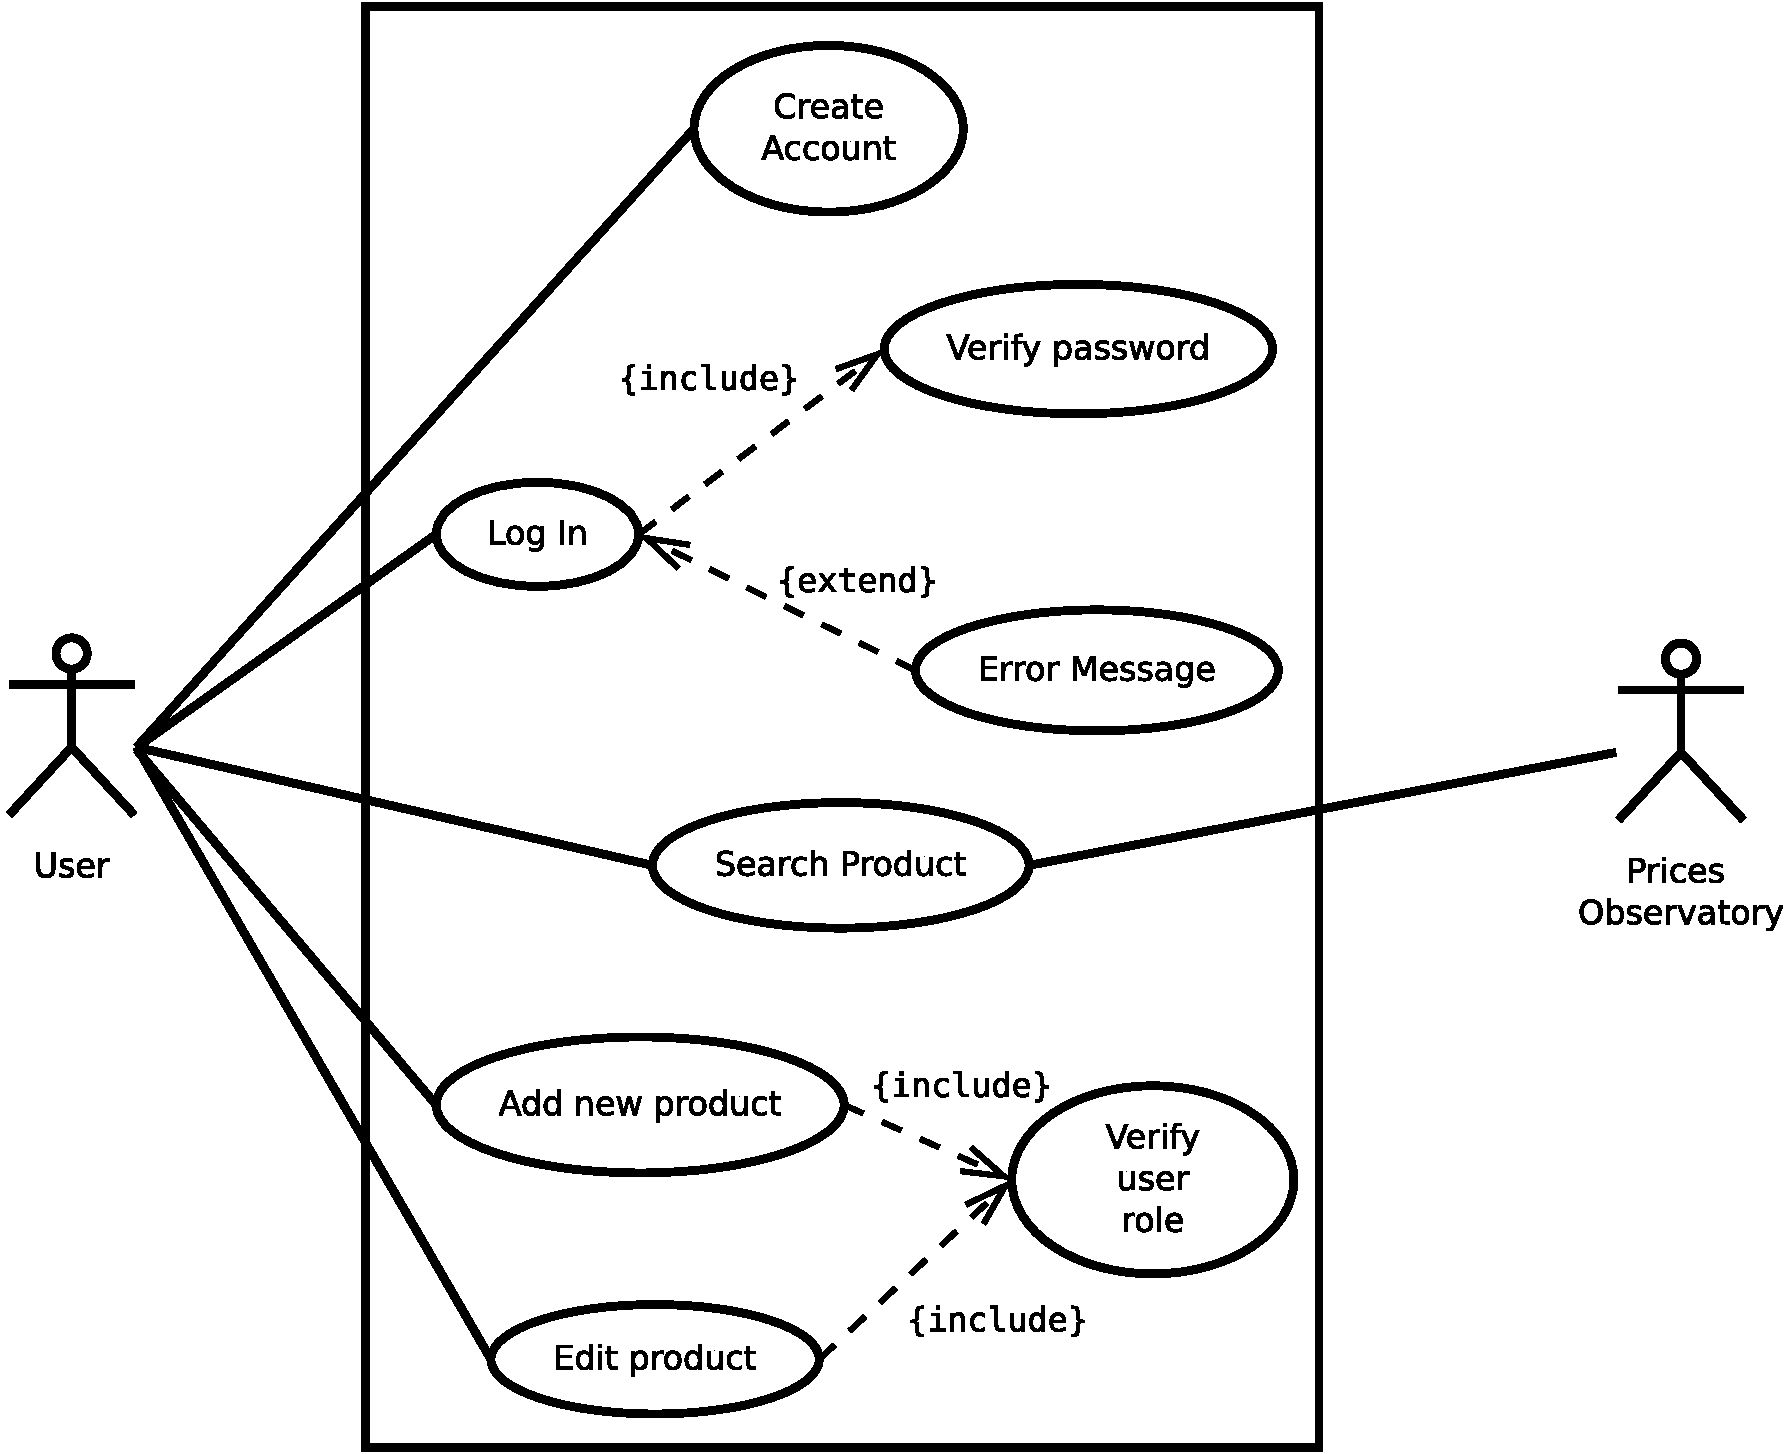
\includegraphics[scale=0.4,keepaspectratio=true]{./user_use_cases.pdf}
   \caption{Το use-case uml διάγραμμα της αλληλεπίδρασης του χρήστη με το παρατηρητήριο τιμών.}
    \label{uml1}
\end{figure}


\textbf{Διαχειριστής Συστήματος}\\
\vspace{0.5cm}
\hspace{0.6cm}Ο διαχειριστής είναι ένας τύπος χρήστη που παίζει καθοριστικό ρόλο όσον αφορά την ασφάλεια και την ομαλή λειτουργία της πλατφόρμας και έχει απόλυτη ελευθερία σχετικά με την επεξεργασία και τη διαχείρισή της. 

\hspace{0.6cm}Ένας από τους ρόλους εξέχουσας σημασίας ενός διαχειριστή είναι να κρίνει αν οι εθελοντές-χρήστες είναι αξιόπιστοι ελέγχοντας τις τιμές που συμπληρώνουν σε κάθε πεδίο (π.χ. αν υπάρχει το όνομα καταστήματος, το όνομα του προϊόντος, αν η τιμή είναι εξωφρενικά μεγάλη για συγκεκριμένο προϊόν). Έτσι, αν κάποιος εθελοντής είναι αξιόπιστος θα συνεχίζει κανονικά να καταχωρεί προϊόντα, ενώ σε αντίθετη περίπτωση θα αναστέλλεται αυτή του η δυνατότητα.

\hspace{0.6cm}Θα μπορεί, επιπροσθέτως, να έχει πρόσβαση στους λογαριασμούς των χρηστών όπου και θα μπορεί να επεξεργάζεται τα προφίλ τους για να αλλάζει τα δικαιώματα και τους ρόλους των χρηστών, μέσα από συγκεκριμένη σελίδα. Ο τρόπος που προστατεύεται η πλατφόρμα είναι επιτρέποντας μόνο σε χρήστες με δικαιώματα διαχειριστή να μπορούν να κάνουν τροποποιήσεις σε αρχεία ή εφαρμογές.

\hspace{0.6cm}Για να τα πραγματοποιήσει όλα αυτά του παρέχεται ξεχωριστός λογαριασμός διαχειριστή με δυνατότητα αναζήτησης χρηστών, πρόσβαση στις πληροφορίες των λογαριασμών τους και δυνατότητα επεξεργασίας τους.

\hspace{0.6cm}Στην εικόνα \ref{uml2} φαίνεται το use-case uml διάγραμμα της αλληλεπίδρασης του διαχειριστή με το σύστημα.

\begin{figure}[H]
   \centering
   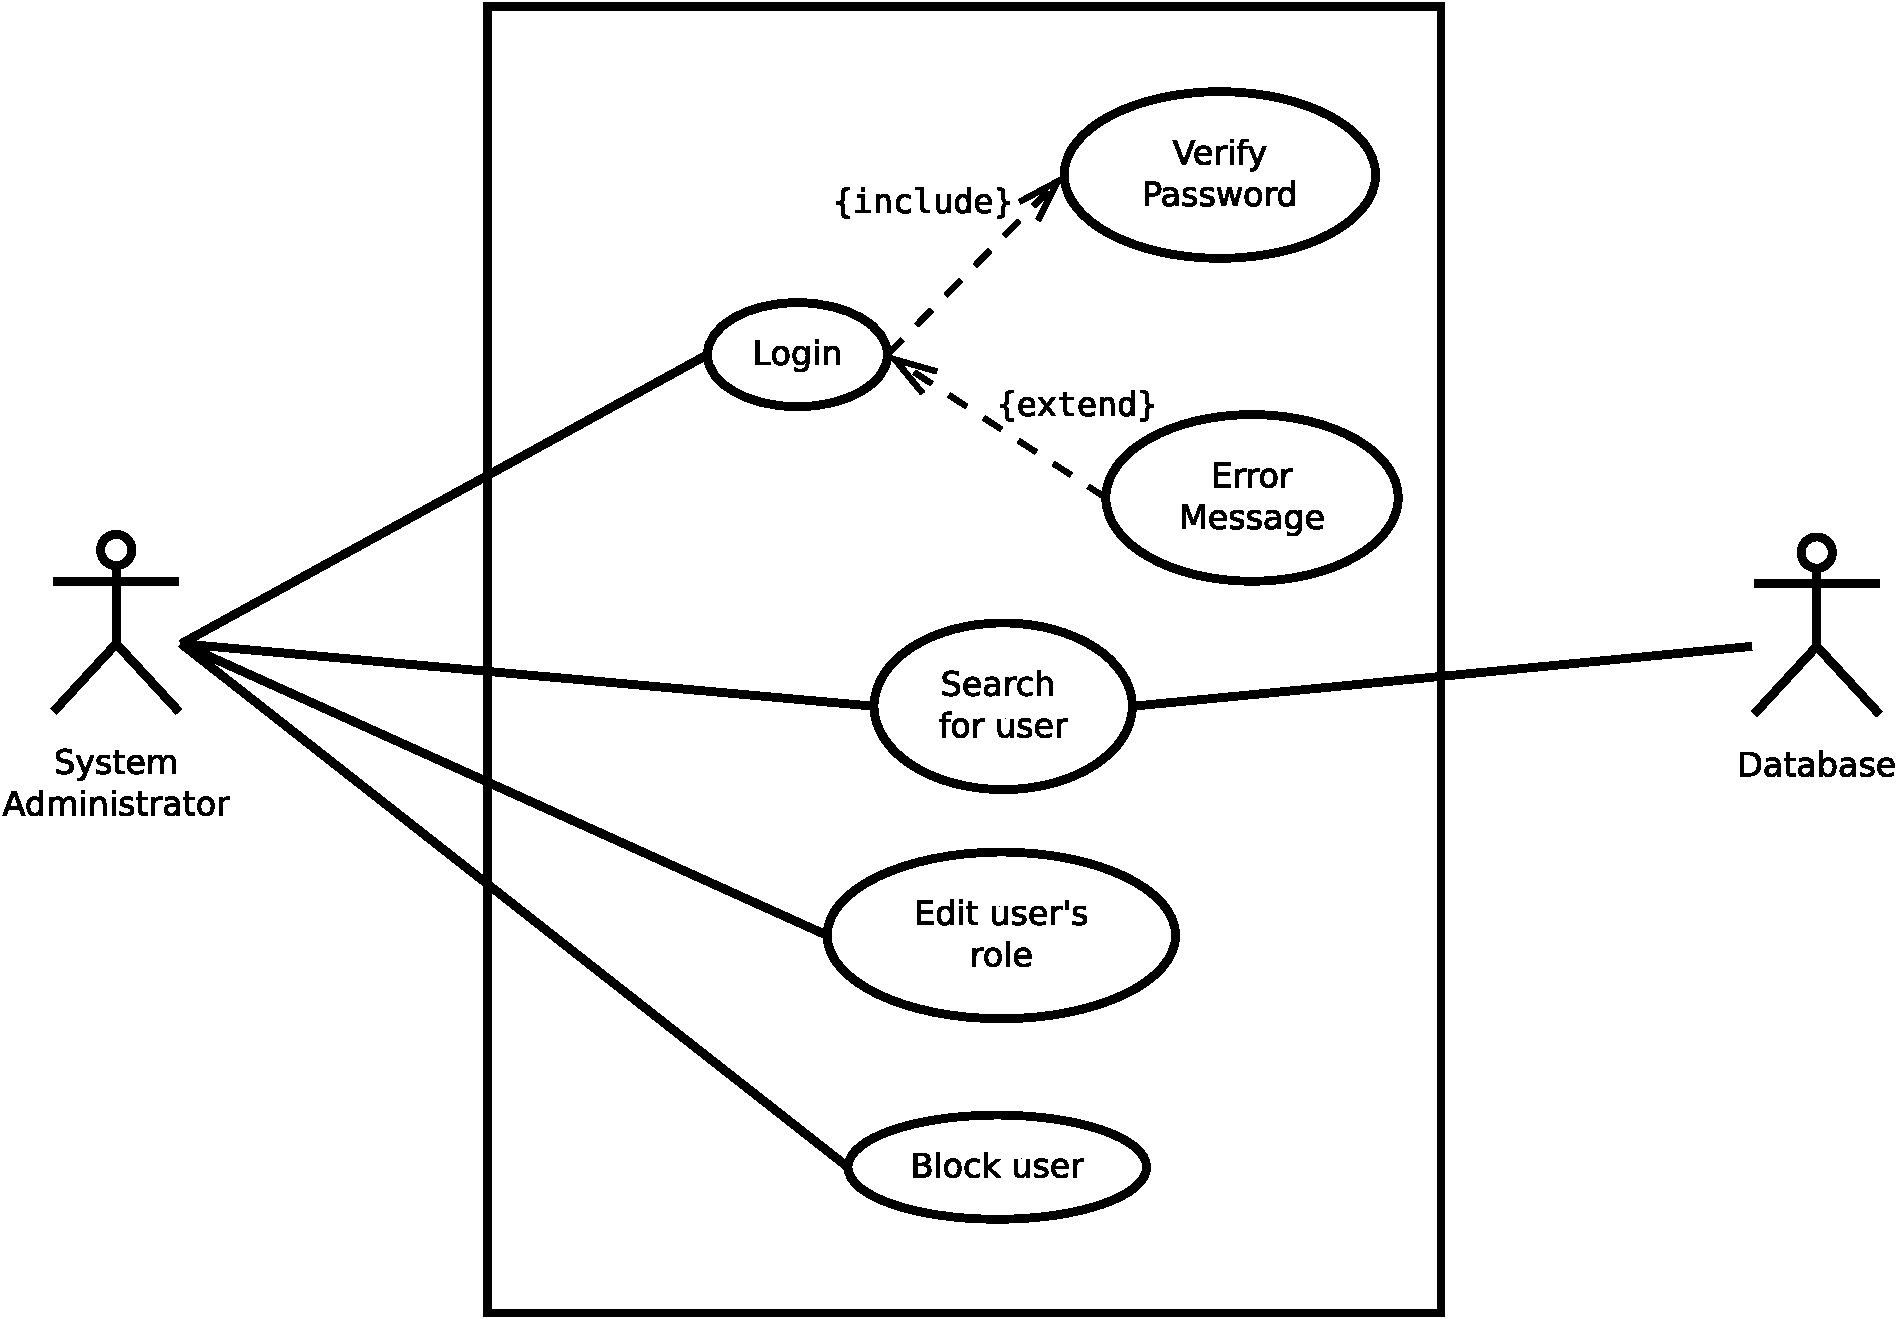
\includegraphics[scale=0.4,keepaspectratio=true]{./admin_use_case.pdf}
   \caption{Το use-case uml διάγραμμα της αλληλεπίδρασης του διαχειριστή συστήματος με την πλατφόρμα του παρατηρητήριο τιμών.}
    \label{uml2}
\end{figure}

\section{Αναφορές - πηγές πληροφοριών}
1)https://www.aiim.org/What-is-Information-Management

\section{Διαχειριστικές απαιτήσεις επιχειρησιακού περιβάλλοντος}

\subsection{Επιχειρησιακό μοντέλο}

\hspace{0.6cm}Η ικανοποίηση των χρηστών είναι απαραίτητη προύπόθεση για την επιτυχία της πλατφόρμας.
Λόγω του ότι είναι άμεσος ο ρόλος των χρηστών εθελοντών κάνει την πλατφόρμα ελκυστική. Τους δίνεται ευκαιρία να ελέγχουν το περιεχόμενο και να ξέρουν ότι τα δεδομένα που βλέπουν είναι έγκυρα. Έτσι τους παρέχεται ένας τρόπος να πάρουν πληροφορίες που θα συνεισφέρουν στη λήψη αποφασεών που είναι πιο συμφέρουσες για μία αγορά. 

\hspace{0.6cm}Η εφαρμογή θα διαδοθεί από χρήστη σε χρήστη ως ένα εργαλείο σχεδιασμένο κυρίως για αυτούς και θα εγκαθιδρυθεί ως ένας βολικός τρόπος έρευνας αγοράς μέσω της συσκευής τους (desktop, tablet, κινητό). Χάρη σ'αυτή θα γλιτώνουν χρόνο αφού δεν θα χρειάζεται να σπαταλάνε ώρες στο δρόμο ψάχνοντας.

\subsection{Περιβάλλον διαχείρισης πληροφοριών}
\hspace{0.6cm}Διαχείριση πληροφοριών είναι η συλλογή και διαχείριση πληροφορίας από διάφορες πηγές και η προσφορά της σε διάφορα κοινά. Ο όρος κοινό περιλαμβάνει τα εμπλεκόμενα μέρη της εφαρμογής διαχείρισης της πληροφορίας και οποιονδήποτε άλλο έχει δικαίωμα πρόσβασης σε αυτή. Ως διαχείριση ορίζεται η οργάνωση και ο έλεγχος στη δομή, την επεξεργασία και διανομή της πληροφορίας.

\hspace{0.6cm}Άρα η διαχείριση πληροφοριών επικεντρώνεται στην ικανότητα ενός οργανισμού να συλλέξει, διαχειριστεί, διατηρήσει, αποθηκεύσει και διανείμει τη σωστή πληροφορία στους σωστούς ανθρώπους, την κατάλληλη στιγμή.

\hspace{0.6cm}Με βάση τη σημερινή εικόνα η διαχείριση πληροφοριών πρέπει να υιοθετεί και να προσκολάτε στις εξής καθοδηγητικές αρχές:
\begin{itemize}
 \item Κάθε αντικείμενο πληροφορίας είναι περιουσιακό στοιχείο της εταιρείας στην οποία ανήκει η πλατφόρμα που το διατηρεί και διαχειρίζεται.
 \item Κάθε πληροφορία της πλατφόρμας πρέπει να είναι διαθέσιμη και να μοιράζεται. Προφανώς δεν γίνεται όλες οι πληροφορίες που διατηρεί η πλατφόρμα να είναι διαθέσιμες προς όλους, για παράδειγμα ευαίσθητες πληροφορίες χρηστών όπως τα passwords. Αλλά κατά γενικό κανόνα πρέπει οι γενικές πληροφορίες να είναι διαθέσιμες προς όλους γιατί προάγει την χρήση της πλατφόρμας και την εκμετάλευση επιχειρηματικής γνώσης.
 \item Η διαχείριση και διατήρησης κάθε πληροφορίας που πρέπει να κρατά πλατφόρμα γίνεται εταιρικά. Αποθηκεύεται και διατηρείται η πληροφορία, δηλαδή ό,τι προσθέτει ο χρήστης τη μία μέρα πρέπει να υπάρχει και την επόμενη.
\end{itemize}

\hspace{0.6cm}Κάθε μέλος της εταιρείας που διαχειρίζεται και συντηρεί την πλατφόρμα είναι υπεύθυνο για την τήρηση των παραπάνω.


\section{Λειτουργικές απαιτήσεις επιχειρησιακού περιβάλλοντος}

\subsection{Επιχειρησιακές διαδικασίες}
\hspace{0.6cm}Η επιχείρησή μας αποτελεί μία διαδικτυακή πλατφόρμα η οποία έχει σχεδιαστεί με σκοπό την προβολή και αγορά κινητών τηλεφώνων σε όσο το δυνατόν χαμηλότερες τιμές.

\hspace{0.6cm}Οι λειτουργικές απαιτήσεις της εφαρμογής μας, από τη μεριά των χρηστών-εθελοντών, είναι να υπάρχει η δυνατότητα καταχώρισης προϊόντος, καταστήματος, χρονικού και χωρικού αποτυπώματος όπως και καταχώριση της τιμής του προϊόντος-κινητού. 

\hspace{0.6cm}Επίσης παρέχουμε τη δυνατότητα να υπάρχουν ανώνυμοι χρήστες. Όσον αφορά αυτούς αλλά και τους χρήστες εθελοντές οι απαιτήσεις είναι να μπορούν να αναζητούν εύκολα και γρήγορα το εκάστοτε προϊόν που ψάχνουν και να λαμβάνουν για αυτό και κάποιες επιπρόσθετες πληροφορίες, όπως κάποιο γράφημα για την εξέλιξη της τιμής του ή τον αριθμό των καταστημάτων στα οποία υπάρχει διαθέσιμο, για κάποια συγκεκριμένη χρονική περίοδο(?).

\hspace{0.6cm}Οι διαχειριστές θα μπορούν να επεξεργάζονται τους λογαριασμούς των χρηστών προκειμένου να αλλάζουν τα δικαιώματα και τους ρόλους τους, μέσα από συγκεκριμένη σελίδα. Επίσης, θα έχουν τη δυνατότητα να διαγράφουν εθελοντές-χρήστες ή να αναστέλλουν την δυνατότητά τους για προσθήκη περαιτέρω προϊόντων, σε περίπτωση που δεν συμμορφώνονται με τους όρους χρήσης ή τα στοιχεία που εισάγουν είναι ανακριβή και ψευδή.

\subsection{Περιορισμοί}

\subsection{Δείκτες ποιότητας}
\hspace{0.6cm}Θα παρέχουμε ασφάλεια δεδομένων όπως και αξιόπιστο δίκτυο καθώς θα κάνουμε χρήση του πρωτοκόλλου HTTPS στην ιστοσελίδα μας. Άλλοι δείκτες ποιότητας είναι η ελάχιστη καθυστέρηση δικτύου (latency) για την ικανοποίηση μιας αίτησης, η συνέπεια των δεδομένων, η διαθεσιμότητα της εφαρμογής, η πιστοποίηση ταυτότητας του εθελοντή-χρήστη καθώς θα κάνει login με μοναδικό username και password, βάση δεδομένων.

\hspace{0.6cm}Τέλος το σύστημα μας θα είναι εύχρηστο διότι κάθε ενέργεια του χρήστη θα είναι πλήρως καθοδηγούμενη. Θα υπάρχουν ευδιάκριτα κουμπιά, πλήρως κατανοητά, και κάθετι που κάνει θα γίνεται με τρόπο που ενδεχομένως να γνωρίζει από αντίστοιχα συστήματα που έχει χρησιμοποιήσει στο παραλθόν.

\section{Έκθεση απαιτήσεων χρηστών}

\textbf{Απαιτήσεις χρηστών-εθελοντών}\\
\vspace{0.5cm}
\hspace{0.6cm}Η διαδικασία εξαγωγής και ανάλυσης των απαιτήσεων των χρηστών κατέληξε στις παρακάτω υψηλού επιπέδου απαιτήσεις που θα υλοποιεί το σύστημα:

\hspace{0.6cm}Οι χρήστες θέλουν να μπορούν να κάνουν αναζητήσεις για προϊόντα που τους ενδιαφέρουν και από τα αποτελέσματα της αναζήτησης να βλέπουν πληροφορίες για το προϊόν που θα επιλέγουν. Οι πληροφορίες αυτές πρέπει να είναι τα ονόματα των καταστημάτων στα οποία έχει καταγραφεί στο παρελθόν, η τελευταία τιμή η οποία έχει καταγραφεί για αυτά σε κάθε κατάστημα, η ημερομηνία και ώρα καταγραφής της τιμής καθώς και η διεύθυνση του καταστήματος σε κείμενο και σημείο στο χάρτη. 

\hspace{0.6cm}Άλλη απαίτηση είναι η προσθήκη νέων προϊόντων και τιμών καθώς και η ενημέρωση υπαρχόντων προϊόντων. Οι πληροφορίες που καταχωρούν θα πρέπει να είναι άμεσα διαθέσιμες σε όλους. Επιπλέον προκειμένου κάθε χρήστης να παρακολουθεί με γρήγορο και εύκολο τρόπο τα προϊόντα που τον ενδιαφέρουν, θα υπάρχει, ενδεχομένως, και μία λίστα αγαπημένων για κάθε λογαριασμό.\\
\vspace{0.5cm}

\textbf{Απαιτήσεις ανώνυμων χρηστών}\\
\vspace{0.5cm}
\hspace{0.6cm}Ως ανώνυμοι χρήστες ορίζονται οι χρήστες της πλατφόρμας οι οποίοι δεν επιθυμούν να δημιουργήσουν λογαριασμό δίνοντας το email τους. Αυτοί οι χρήστες θέλουν να αναζητού και να  έχουν πρόσβαση στα προϊόντα που υπάρχουν στο σύστημα, δηλαδή, να βλέπουν τα αποτελέσματα και το προφίλ του κάθε προϊόντος. Συνεπώς θέλουν μόνο να ενημερώνονται για τις τιμές των προϊόντων χωρίς να χρειάζεται να είναι εγγεγραμένοι.\\
\vspace{0.5cm}

\textbf{Απαιτήσεις διαχειριστών συστήματος}\\
\vspace{0.5cm}
\hspace{0.6cm}Οι διαχειριστές συστήματος απαιτούν να έχουν άνετη πρόσβαση μέσω της πλατφόρμας στο backend σύστημα για να διαχειρίζονται τους λογαριασμούς των χρηστών. Θέλουν να έχουν πρόσβαση στους λογαριασμούς κάθε χρήστη και να μπορούν να τους επεξεργαστούνν, να αλλάζουν τους ρόλους των χρηστών και να μπλοκάρουν χρήστες που θεωρούν ότι βλάπτουν την καλή λειτουργία του συστήματος και την ασφάλεια των άλλων χρηστών. 

\section{Αρχές του προτεινόμενου συστήματος}

\textbf{Χρήστης}\\
\vspace{0.5cm}
\hspace{0.6cm}Το προτεινόμενο σύστημα θα έχει τις εξής λειτουργικές αρχές:
\begin{enumerate}
 \item Δυνατότητα δημιουργίας λογαριασμού χρήστη δίνοντας email, username και password.
 \item Δυνατότητα εισόδου ως χρήστης εισάγωντας τα email και password που ορίστηκαν κατά την εγγραφή του χρήστη.
 \item Δυνατότητα ανάκτησης password σε περίπτωση που ο χρήστης το ξέχασε.
 \item Δυνατότητα αναζήτησης προϊόντων με χρήση της μπάρας αναζήτησης που θα υπάρχει σε κάθε σελίδα που μπορεί να βρεθεί ο χρήστης.
 \item Λίστα αποτελεσμάτων αναζήτησης από όπου θα μπορεί ο χρήστης να επιλέξει όποιο προϊόν επιθυμεί.
 \item Μοναδικό προφίλ για κάθε προϊόν το οποίο θα περιλαμβάνει:
    \begin{enumerate}
     \item Όλα τα καταστήματα όπου είναι διαθέσιμο το προϊόν οργανωμένα σε δικούς τους <<τομείς>>.
     \item Η τελευταία τιμή η οποία καταγράφηκε για το αντίστοιχο κατάστημα.
     \item Η ημερομηνία καταχώρησης της τελευταίας τιμής.
     \item Η διεύθυνση του αντίστοιχου καταστήματος.
     \item Χάρτης όπου θα φαίνεται το στίγμα της τοποθεσίας του καταστήματος.
     \item Κουμπί επεξεργασίας δίπλα σε κάθε κατάστημα για προσθήκη νέας τιμής.
     \item Κουμπί για προσθήκη νέου καταστήματος.
     \item Πίνακας με στατιστικά στοιχεία της διακύμανσης της τιμής.
    \end{enumerate}
\item Δυνατότητα προσθήκης νέου προϊόντος μέσω αντίστοιχου κουμπιού που οδηγεί σε φόρμα εισαγωγής στοιχείων του προϊόντος, όπου θα ζητηθούν τα εξής:
    \begin{enumerate}
     \item Μήνυμα ενεργοποίησης gps εφόσον ο χρήστης το επιθυμεί.
     \item Δεδομένου ότι το gps είναι ενεργό τότε θα εντοπίζεται η τοποθεσία του χρήστη και θα συμπληρώνεται η διεύθυνση του καταστήματος.
     \item Εισαγωγή ονόματος προϊόντος.
     \item Εισαγωγή ονόματος καταστήματος.
     \item Εισαγωγή τιμής σε \texteuro.
     \item Εισαγωγή διεύθυνσης καταστήματος αν ο χρήστης δεν επιλέξει να ενεργοποιήσει το gps της συσκευής του.     
    \end{enumerate}
\item Το χρονικό αποτύπωμα του χρήστη θα λαμβάνεται σε όλες τις περιπτώσεις αυτόματα από το ρολόι του συστήματος της συσκευής του.
\item Διατήρηση λίστας για κάθε χρήστη αγαπημένων προϊόντων στην οποία θα μπορεί να προσθέτει και να αφαιρεί όποιο προϊόν θέλει.
\item Δυνατότητα αποσύνδεσης.
\end{enumerate}

\vspace{0.5cm}
\textbf{Σενάριο 1-Αποτυχημένη αναζήτηση προϊόντος}\\
\begin{enumerate}
 \item Ο  ανώνυμος χρήστης ανοίγει την αρχική σελίδα και πληκτρολογεί το όνομα του προϊόντος στην μπάρα αναζήτησης.
 \item Το αντικείμενο δεν βρέθηκε και εμφανίζεται μήνυμα αποτυχίας με δυνατότητα αναζήτησης νέου προϊόντος.
\end{enumerate}

\vspace{0.5cm}
\textbf{Σενάριο 2-Επιτυχημένη αναζήτηση προϊόντος}\\
\begin{enumerate}
 \item Ο  ανώνυμος χρήστης ανοίγει την αρχική σελίδα και πληκτρολογεί το όνομα του προϊόντος στην μπάρα αναζήτησης.
 \item Το αντικείμενο βρέθηκε και εμφανίζονται τα μαγαζιά στα οποία υπάρχει και οι αντίστοιχες τιμές που έχει κάθε κατάστημα.
\end{enumerate}

\vspace{0.5cm}
\textbf{Σενάριο 3-Προσθήκη καινούργιας τιμής-καταστήματος σε υπάρχον προϊόν}\\
\begin{enumerate}
 \item Ο χρήστης ανοίγει την αρχική σελίδα και πληκτρολογεί το όνομα του προϊόντος στην μπάρα αναζητήσης.
 \item Το αντικείμενο βρέθηκε και εμφανίζονται τα μαγαζιά στα οποία υπάρχει και οι αντίστοιχες τιμές που έχει κάθε κατάστημα.
 \item Μπορεί να τροποποιήσει την τιμή που έχει το προϊόν σε κάποιο κατάστημα μέσω αντίστοιχου κουμπιού επεξεργασίας της τιμής ή να προσθέσει καινούργιο κατάστημα το οποίο δεν είναι καταχωρημένο ότι παρέχει το προϊόν, μέσω κουμπιού προσθήκης προϊόντος.
 \item Αν ο χρήστης δεν είναι συνδεδεμένος ήδη το πάτημα ενός εκ των δύο κουμπιών ρωτάει τον χρήστη αν έχει λογαριασμό ή αν επιθυμεί να δημιουργήσει στην περίπτωση που δεν διαθέτει.
 \begin{itemize}
  \item Ο ήδη εγγεγραμμένος χρήστης συμπληρώνει το email και το password του.
  \item Αν ο εγγεγραμμένος χρήστης εισάγει λάθος password εμφανίζεται μήνυμα αποτυχίας και του δίνεται η  δυνατότητα να ξανά εισάγει το password ή να πατήσει ότι το ξέχασε και να εκκινήσει διαδικασία ανάκτησης.
  \item O μη εγγεγραμμένος συμπληρώνει σε διπλανή φόρμα το email, username και κάποιο password που επιθυμεί.
 \end{itemize}

 \item  Επιτυχής σύνδεση οδηγεί σε φόρμα προσθήκης νέου προϊόντος όπου ο χρήστης συμπληρώνει το όνομα του, το όνομα του καταστήματος και την τιμή του, στην περίπτωση εισαγωγής προϊόντος σε κατάστημα που δεν υπάρχει καταχωρημένο. Αλλιώς, του εμφανίζεται η υπάρχουσα τιμή του προϊόντος σε συγκεκριμένο κατάστημα με δυνατότητα επεξεργασίας της τιμής.
 
 \item Εφόσον ο χρήστης το επιθυμεί, ανοίγοντας το gps του λαμβάνεται αυτόματα η τοποθεσία του ως διεύθυνση του καταστήματος, στην περίπτωση εισαγωγής προϊόντος σε κατάστημα που δεν υπάρχει καταχωρημένο.
 \item Πατώντας το κουμπί αποθήκευσης ο χρήστης οδηγείτε στο προφίλ του προϊόντος όπου φαίνεται η νέα καταχώρηση καταστήματος-τιμής ή η νέα-ανανεωμένη τιμή του προϊόντος σε υπάρχον κατάστημα, η ημερομηνία και ώρα καταχώρησης, τις οποίες πρόσθεσε το σύστημα αυτόματα από τη συσκευή του χρήστη, και ο χάρτης με την τοποθεσία του καταστήματος. 
\end{enumerate}

\vspace{0.5cm}
\textbf{Σενάριο 4-Προσθήκη νέου προϊόντος}\\
\begin{enumerate}
 \item Ο χρήστης ανοίγει την αρχική σελίδα και πληκτρολογεί το όνομα του προϊόντος στην μπάρα αναζητήσης.
 \item Το αντικείμενο δεν βρέθηκε και εμφανίζεται μήνυμα αποτυχίας και η επιλογή μέσω κουμπιού προσθήκης νέου προϊόντος
 \item Αν ο χρήστης δεν είναι συνδεδεμένος ήδη το πάτημα του κουμπιού ρωτάει τον χρήστη αν έχει λογαριασμό ή αν επιθυμεί να δημιουργήσει στην περίπτωση που δεν διαθέτει.
 \begin{itemize}
  \item Ο ήδη εγγεγραμμένος χρήστης συμπληρώνει το email και το password του.
  \item Αν ο εγγεγραμμένος χρήστης εισάγει λάθος password εμφανίζεται μήνυμα αποτυχίας και του δίνεται η  δυνατότητα να ξανά εισάγει το password ή να πατήσει ότι το ξέχασε και να εκκινήσει διαδικασία ανάκτησης.
  \item O μη εγγεγραμμένος συμπληρώνει σε διπλανή φόρμα το email, username και κάποιο password που επιθυμεί.
 \end{itemize}
 \item Επιτυχής σύνδεση οδηγεί σε φόρμα προσθήκης νέου προϊόντος όπου ο χρήστης συμπληρώνει το όνομα του, το όνομα του καταστήματος και την τιμή του.
 \item Εφόσον ο χρήστης το επιθυμεί και ανοίγοντας το gps του λαμβάνεται αυτόματα η τοποθεσία του ως διεύθυνση του καταστήματος. Αλλιώς την εισάγει με το χέρι.
 \item Πατώντας το κουμπί αποθήκευσης ο χρήστης οδηγείτε στο προφίλ του προϊόντος όπου φαίνεται η νέα καταχώρηση καταστήματος-τιμής, η ημερομηνία και ώρα καταχώρησης, τις οποίες πρόσθεσε το σύστημα αυτόματα από τη συσκευή του χρήστη, και ο χάρτης με την τοποθεσία του καταστήματος.
\end{enumerate}

\vspace{0.5cm}
\textbf{Διαχειριστής συστήματος}\\
\vspace{0.5cm}
Το προτεινόμενο σύστημα θα έχει τις εξής λειτουργικές αρχές:
\begin{enumerate}
 \item Δυνατότητα εισόδου ως διαχειριστής δίνοντας username και password.
 \item Δυνατότητα ανάκτησης password σε περίπτωση που ο διαχειριστής το ξέχασε.
 \item Δυνατότητα αναζήτησης λογαριασμών χρηστών μέσω μπάρας αναζήτησης.
 \item Δυνατότητα επισκόπησης των στοιχείων των λογαριασμών χρηστών με τη μορφή πίνακα.
 \item Δυνατότητα επεξεργασίας του ρόλου κάθε χρήστη μέσω κουμπιού edit.
 \item Δυνατότητα μπλοκαρίσματος/διαγραφής κάποιου χρήστη με χρήση κουμπιού διαγραφής.
\end{enumerate}

\vspace{0.5cm}
\textbf{Σενάριο 1-Αλλαγή ρόλων χρηστών}
\begin{enumerate}
 \item  Ο διαχειριστής ανοίγει την αρχική σελίδα και κάνει login χρησιμοποιώντας το email και τον κωδικό του.
 \item Αν εισάγει λάθος password εμφανίζεται μήνυμα αποτυχίας και του δίνεται η δυνατότητα να ξανά εισάγει το password ή να πατήσει ότι το ξέχασε και να εκκινήσει διαδικασία ανάκτησης.
 \item Μετά την επιτυχή σύνδεση, οδηγείται σε σελίδα όπου μπορεί να δει όλα τα προφίλ των χρηστών σε βολική μορφή, καθένα από τα οποία θα έχει κάποιες επιλογές, μέσω κατάλληλων κουμπιών, για διαγραφή χρήστη ή αλλαγή ρόλων χρήστη. 
 \item Στην ίδια σελίδα υπάρχει μπάρα αναζήτησης για να βρίσκει γρήγορα συγκεκριμένους χρήστες.
 \item Έτσι θα μπορεί να διαγράψει κάποιον χρήστη αν οι πράξεις του δεν συνάδουν με τους όρους χρήσης της εφαρμογής ή αν συμπληρώνει αναληθή δεδομένα, μέσω κουμπιού διαγραφής χρήστη. Επίσης, θα μπορεί να αλλάξει τον ρόλο κάποιου χρήστη και να τον κάνει π.χ. και αυτόν διαχειριστή, σε περίπτωση που το κρίνει χρήσιμο, μέσω κουμπιού αλλαγής ρόλου χρήστη.
\end{enumerate}


s\ection{Περιορισμοί στο πλαίσιο του έργου}
\textbf{Χρήστης}\\
\vspace{0.5cm}
\hspace{0.6cm}Κανένας χρήστης δεν θα μπορεί να δει τους λογαριασμούς των άλλων χρηστών και επομένως δεν θα έχουν τη δυνατότητα ούτε να διαγράψουν κάποιον χρήστη, ούτε να αλλάξουν το ρόλο, ούτε οποιοδήποτε άλλο στοιχείο των προσωπικών δεδομένων των υπολοίπων χρηστών. Επίσης κανένας χρήστης δεν θα μπορεί να διαγράψει προϊόντα ως οντότητες ούτε να αλλάξει στοιχεία τους πέρα από τα προβλεπόμενα. Δεν θα είναι δυνατή η εγγραφή χρηστών με ίδιο email ούτε με ίδιο username, διότι αυτά θα θεωρούνται μοναδικά από το σύστημα. 

\hspace{0.6cm}Δεν θα είναι δυνατό να εμφανίζεται για κάποιο προϊόν το ίδιο κατάστημα πάνω από μία φορά με ίδια ή διαφορετική τιμή. Μετά την εισαγωγή νέων τιμών οι παλαιότερες τιμές δεν θα φαίνονται παρα μόνο σαν στατιστικό στοιχείο στον αντίστοιχο πίνακα.\\

\vspace{0.5cm}
\textbf{Ανώνυμοι Χρήστες}\\
\vspace{0.5cm}
\hspace{0.6cm}Οι μη εγγεγραμμένοι χρήστες θα μπορούν μόνο να αναζητούν προϊόντα και δεν θα έχουν κανένα από τα προνόμια που έχουν οι εγγεγραμένοι χρήστες (προσθήκη προϊόντων, επεξεργασία τιμής προϊόντων).\\

\vspace{0.5cm}
\textbf{Διαχειριστές}\\

\hspace{0.6cm}Οι διαχειριστές δεν έχουν εν γένει περιορισμούς εκτός από το γεγονός ότι δεν θα μπορούν να βλέπουν ή να εντοπίζουν με κάποιον τρόπο τους κωδικούς των εγγεγραμμένων χρηστών.
% 
% Σε περίπτωση αστοχίας του δικτύου, μας ενδιαφέρει πιο πολύ η διαθεσιμότητα της εφαρμογής παρά (η συνέπεια των δεδομένων) η πιο πρόσφατη ενημέρωση κάποιου προϊόντος. Επίσης, σε περίπτωση αστοχίας του δικτύου μας ενδιαφέρει πιο πολύ η ελαχιστοποίηση της καθυστέρησης στην απόκριση του συστήματος παρά (η συνέπεια των δεδομένων) η πιο πρόσφατη ενημέρωση κάποιου προϊόντος. Αν βέβαια δεν υπάρχει αστοχία δικτύου, θα προτιμήσουμε συνέπεια δεδομένων.


\section{Παράρτημα: ακρωνύμια και συντομογραφίες}




\end{document}
